\documentclass{gnulike}

\usepackage{natbib}
\usepackage{graphics}
\usepackage{chngcntr}
\usepackage{sectsty}
\usepackage{rotating}
\usepackage{emptypage}
\usepackage[titletoc]{appendix}
\usepackage{multicol}

\let\leqslant=\leq

\DeclareMathSizes{10}{10}{10}{10}

\definecolor{light-gray}{gray}{0.95}
\definecolor{bashgray}{RGB}{211,215,207}
\definecolor{bashgray2}{RGB}{238,238,236}
\newcommand{\addbash}[1]{
	\begin{center}
	\fcolorbox{aluminium3}{aluminium1}{\begin{minipage}{0.9\textwidth}
  	\ttfamily \$ #1
\end{minipage}}
	\end{center}
}

\newcommand{\addbox}[1]{
	\begin{center}
	\fcolorbox{aluminium3}{aluminium1}{\begin{minipage}{0.98\columnwidth}
  	#1
        \end{minipage}}
	\end{center}
}

\renewcommand{\theequation}{\arabic{equation}}
\renewcommand{\thefigure}{\arabic{figure}}

\usepackage[dvipsnames]{xcolor}
\usepackage{minibox}

\usepackage{graphicx}
\usepackage{color}

\newcommand{\indice}[1]{\scriptsize{#1}}
\newcommand{\subtitle}{FDPSV}

\titleformat{\chapter}[hang] 
{\normalfont\huge\bfseries}{\thechapter}{0.5em}{} 
\titlespacing*{\chapter}{0pt}{-20pt}{20pt}

\usepackage{makeidx}
\makeindex

\mdseries

\begin{document}

\begin{titlepage}
  \newpage
  \null
  \vskip 10.0em
  \let\center\flushleft
  {\noindent \huge{\bf SWAM2D} \par}
  \vskip -0.5em
  {\noindent \rule{\textwidth}{0.3em} \par}

  {\hfill Documentation for SWAM2D version 1.0.0-rc \par}
  
  {\hfill 26 January 2017 \par}
  
  \vfill
  
  {\noindent \Large{Damien Pageot}}
  \vskip -0.5em
  {\noindent \rule{\textwidth}{0.2em} \par}
  \vskip 1.0cm
\end{titlepage}

% ----------------------------------------------------------------------
% COPYING (MANUAL)
% ----------------------------------------------------------------------
\null\vfill
\thispagestyle{empty}
\pagenumbering{gobble}

\noindent Copyright \copyright\ 2016-2017 Damien Pageot.\\

\noindent Permission is granted to copy, distribute and/or modify this document under the terms of the GNU Free Documentation License, Version 1.3 or any later version published by the Free Software Foundation; with no Invariant Sections, no Front-Cover Texts, and no Back-Cover Texts. A copy of the license is included in the section entitled "GNU Free Documentation License".

\clearpage\newpage


% ----------------------------------------------------------------------
% TABLE OF CONTENTS
% ----------------------------------------------------------------------
\pagenumbering{roman}
\tableofcontents
\thispagestyle{empty}
\clearpage\newpage

\pagenumbering{arabic}

% ----------------------------------------------------------------------
% INTRODUCTION
% ----------------------------------------------------------------------
\chapter{Introduction}
\index{Introduction}

% ----------------------------------------------------------------------
% THEORETICAL BACKGROUND
% ----------------------------------------------------------------------
\chapter{Method}

\section{Governing equation}
\index{governing equation}

\noindent The equation of motion in an elastic medium can be written, in its compact formulation, as (\cite{aki2002quantitative}, \cite{virieux2016modelling}):

\begin{equation}
  \label{eq:motion}
  \rho(x) \frac{\partial^{2}u_{i}}{\partial t^{2}} = \frac{\partial \sigma_{ik}}{\partial x_{k}} + \rho(x)f_{i} ,
\end{equation}

\noindent where $x=(x,y,z)$ is the position vector, $u$ is the displacement, $\sigma_{ij}$ is the stress tensor, $\rho(x)$ is the density and $f=(f_{x}, f_{y}, f_{z})$ is the a volumetric force.\\

\noindent The stress tensor $\sigma$, which allows to describe the elastic medium, is lineary relied to the strain tensor $\epsilon$ through the fourth-rank elastic tensor $C_{ijkl}$. This linear relation, called generalized Hooke's law,  is defined as follow:

\begin{equation}
  \label{eq:hooke}
  \sigma_{ij} = C_{ijkl}\epsilon_{kl}\ ,
\end{equation} 

\noindent where

\begin{equation}
  \label{eq:elastic-tensor}
  C_{ijkl} = \lambda \delta_{ij} \delta_{kl} + \mu (\delta_{ik}\delta_{jl}+\delta_{il}\delta_{jk})\ ,
\end{equation}

\noindent where $\delta$ is the Kronehker symbol and $\lambda$ and $\mu$ are the Lam\'e parameters.\\

\noindent The strain tensor corresponds to the symetric part of the displacement derivatives with respect to space, \textit{i.e.} to the deformation of the elastic body such as:

\begin{equation}
  \label{eq:strain-tensor}
  \epsilon_{ij} = \frac{1}{2} \left( \frac{\partial u_{j}}{\partial x_{i}} + \frac{\partial u_{i}}{\partial x_{j}} \right)\ .
\end{equation}

\noindent Combining equations \ref{eq:hooke}, \ref{eq:elastic-tensor} and \ref{eq:strain-tensor}, and injecting the result in equation \ref{eq:motion} leads to the second order hyperbolic system, called displacement-stress formulation. In 2D, where all derivative with respect to $y$ vanishes, the displacement-stress formulation is:

\index{displacement-stress formulation}
\begin{eqnarray}
  \label{eq:displacement-stress}
  \frac{\partial ^{2} u_{x}}{\partial t^{2}} = \rho^{{\scriptscriptstyle-1}} \left( \frac{\partial \sigma_{xx}}{\partial x} + \frac{\partial \sigma_{xz}}{\partial z} \right)\ , \nonumber \\
  \frac{\partial ^{2} u_{z}}{\partial t^{2}} = \rho^{{\scriptscriptstyle -1}} \left( \frac{\partial \sigma_{xz}}{\partial x} + \frac{\partial \sigma_{zz}}{\partial z} \right)\ ,
\end{eqnarray}

\noindent where:

\begin{eqnarray}
  \label{eq:displacement-stress-2}
  \sigma_{xx} = (\lambda+2\mu)\frac{\partial u_{x}}{\partial x} + \lambda \frac{\partial u_{z}}{\partial z}\ , \nonumber \\
  \sigma_{zz}= (\lambda+2\mu)\frac{\partial u_{z}}{\partial z} + \lambda \frac{\partial u_{x}}{\partial x}\ , \\
  \sigma_{xz} = \mu \left( \frac{\partial u_{x}}{\partial z} + \frac{\partial u_{z}}{\partial x } \right)\ . \nonumber
\end{eqnarray}\\

\noindent This system can be expressed in term of velocity instead of displacement which leads to the first-order hyperbolic system, called velocity-stress formulation:

\index{velocity-stress formulation}
\begin{eqnarray}
  \label{eq:velocity-stress}
  \frac{\partial v_{x}}{\partial t} = \rho^{{\scriptscriptstyle-1}} \left( \frac{\partial \sigma_{xx}}{\partial x} + \frac{\partial \sigma_{xz}}{\partial z} \right) \nonumber \\
  \frac{\partial v_{z}}{\partial t} = \rho^{{\scriptscriptstyle -1}} \left( \frac{\partial \sigma_{xz}}{\partial x} + \frac{\partial \sigma_{zz}}{\partial z} \right) \nonumber \\
  \frac{\partial \sigma_{xx}}{\partial t} = (\lambda+2\mu)\frac{\partial v_{x}}{\partial x} + \lambda \frac{\partial v_{z}}{\partial z} \\
  \frac{\partial \sigma_{zz}}{\partial t} = (\lambda+2\mu)\frac{\partial v_{z}}{\partial z} + \lambda \frac{\partial v_{x}}{\partial x} \nonumber \\
  \frac{\partial \sigma_{xz}}{\partial t} = \mu \left( \frac{\partial v_{x}}{\partial z} + \frac{\partial v_{z}}{\partial x } \right) \nonumber
\end{eqnarray}

\section{Staggered-grid scheme}
\index{staggered-grid scheme}

\cite{virieux1986psv,levander1988fourth,bohlen2006accuracy}

\begin{figure}[!ht]
  \centering
  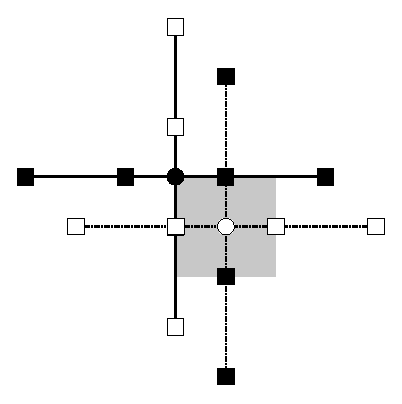
\includegraphics[width=0.9\textwidth]{fig/staggered.eps}
  \caption{Staggered finite-difference grid and spatial stencils for (a) the velocity update and (b) the stress update. After \cite{levander1988fourth} with velocity-stress position switch proposed by \cite{bohlen2006accuracy}.}
  \label{fig:staggered-grid}
\end{figure}

\section{Discretization}

\noindent Given the use of the staggered-grid scheme to discretize the space, forward and backward finite-difference operators are use to solve the velocity-stress equations.\\

%\noindent Second order forward ($D^{+}$) and backward ($D^{-}$) operators:
%\index{forward operator}
%\index{backward operator}
%\begin{eqnarray}
%  D^{+}=f(i+1)-f(i) \nonumber \\
%  D^{-}=f(i)-f(i-1)
%\end{eqnarray}

\noindent The fourth-order forward ($D^{+}$) and backward ($D^{-}$) operators are widely used and are defined, in 1D, as:
\index{forward operator}
\index{backward operator}

\begin{eqnarray}
  D^{+}=c_{1}[f(i+1)-f(i)]+c_{2}[f(i+2)-f(i-1)] \nonumber \\
  D^{-}=c_{1}[f(i)-f(i-1)]+c_{2}[f(i+1)-f(i-2)]
\end{eqnarray}


\index{Lam\'e parameters}
\index{parameter harmonization}
\begin{eqnarray}
  \bar{\mu}(i+\frac{1}{2}, j+\frac{1}{2})=\frac{1}{4}(\mu(i,j)+\mu(i+1,j)+\mu(i,j+1)+\mu(i+1,j+1) \\
  \rho_{x}(i,j+\frac{1}{2}) = \frac{1}{2}(\rho (i,j+1)+\rho(i,j)) \\
  \rho_{z}(i+\frac{1}{2},j) = \frac{1}{2}(\rho (i+1,j)+\rho(i,j))
\end{eqnarray}

\clearpage\newpage
\begin{figure}[!ht]
  \centering
  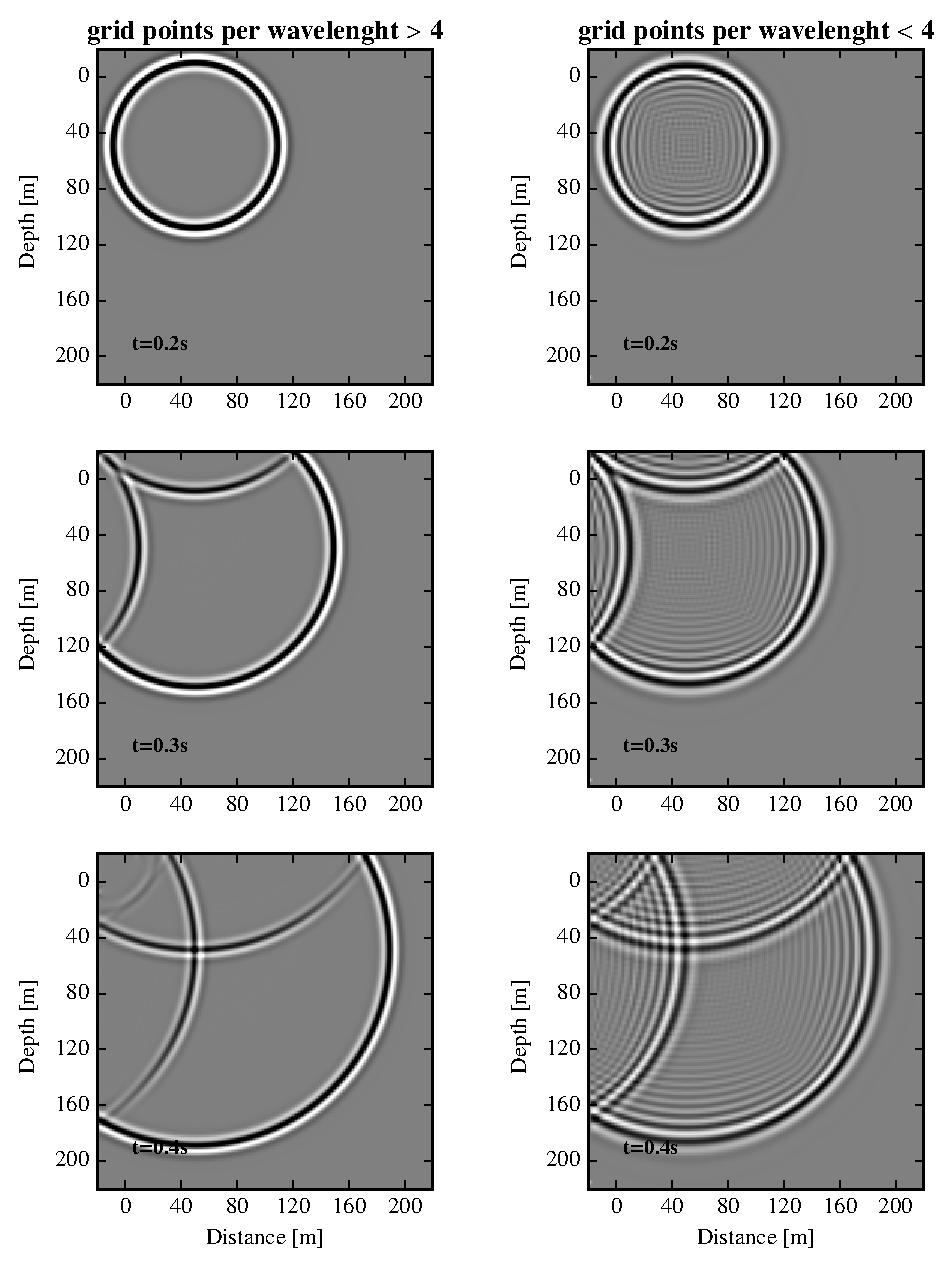
\includegraphics[scale=1.0]{fig/validation_dispersion.eps}
  \caption{Comparison between (left) a modeling using a suitable number of grid points per wavelenght and (right) a modeling using unsufficient nomber of grid points per wavelenght.}
  \label{fig:dispersion-validation}
\end{figure}

\begin{figure}[!ht]
  \centering
  \includegraphics[scale=1.0]{fig/validation_courant.eps}
  \caption{.}
  \label{fig:courant-validation}
\end{figure}

\section{Initial and boundary conditions}
\index{absorbing boundary condition}
\index{free surface condition}

\subsection{PML absorbing boundary conditions}
\index{perfectly matched layer}
\index{absorbing boundary conditions}

\noindent At the scale of seismic exploration and less, the target area (\textit{i.e.} the model), is a semi-infinite space bounded only at the top by a free surface. It is thus necessary to simulate a infinite medium at the lateral and bottom boundary. This can be achieve using the \textit{Perfectly matched layer} (PML) absorbing boundaries. PML were initially developed in the framework of electro-magentic modeling by \cite{berenger1994perfectly} and was quickly adopted in seismic modeling.\\

\noindent In the time domain, PML can be defined as:

\begin{eqnarray}
\label{eq:pml-equations}
d = d_{0} \left( \frac{q}{L_{PML}} \right) ^{n}\ , \\
d_{0} = Ac_{p} \frac{log(1/R)}{2L_{PML}}\ ,
\end{eqnarray}

\noindent where $q$ is the distance from PML intern boundary, $L_{PML}$ is the width of the PML, $A$ is the amplitude of the PML, $c_{p}$ is the P-wave velocity and $R$ is a reflection coefficient generally low.\\

\noindent Figure \ref{fig:validation-pml} demonstrate the importance of absorbing boundary conditions and the efficiency of PML. PML are parametrized following recommandations of (CITE KOMATITSCH, FESTA HERE): $A=3$ and $R=0.01$. In this example, the PML are $20\ m$ wide (40 grid points).
\begin{figure}[!ht]
  \centering
  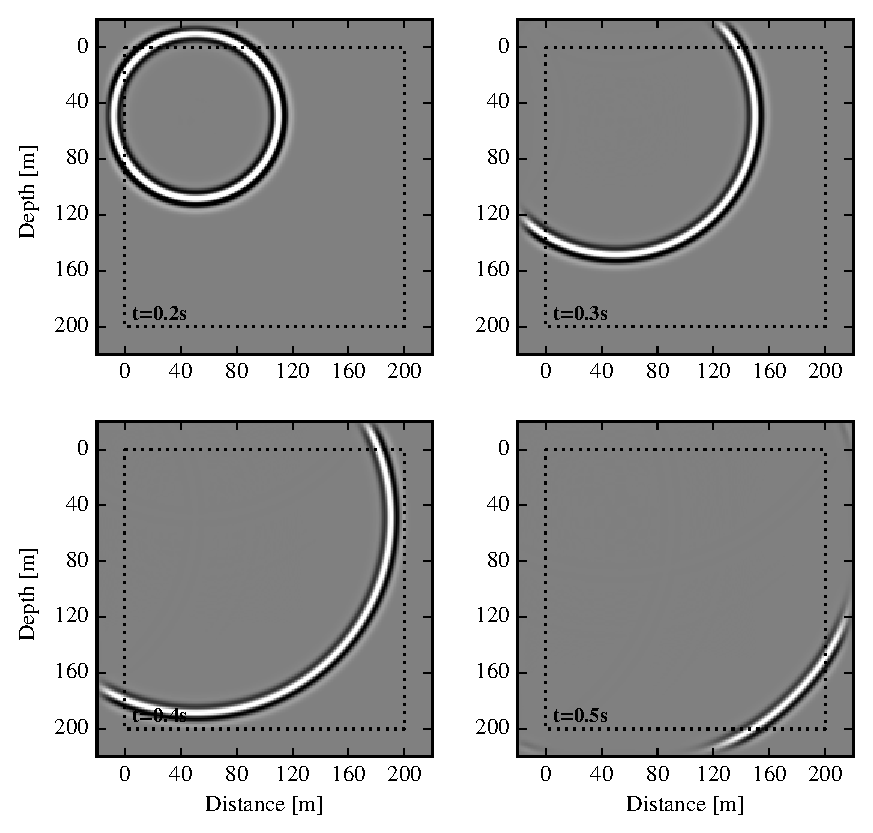
\includegraphics[scale=1.0]{fig/validation_pml.eps}
  \caption{Comparison of (left column) snapshots of the pressure wavefield for a model without PML ($A=0$) and (right column) snapshots of the pressure wavefield for a model with PML ($A=3$) applied to each boundary. Black dashed line defined the limits between PML and physical model.}
  \label{fig:validation-pml}
\end{figure}

\subsection{Free surface}
\index{free surface}

\noindent As discussed in the previous subsection, the earth structures must be considered as semi-infite space due to the presence of a free surface defined by the topography. Given the strong formulation of the wave equation used by finite-difference methods, the free surface must be explicitly defined.\\

\noindent Two popular methods are the vaccum approach and the image theory approach.

\begin{figure}[!ht]
  \centering
  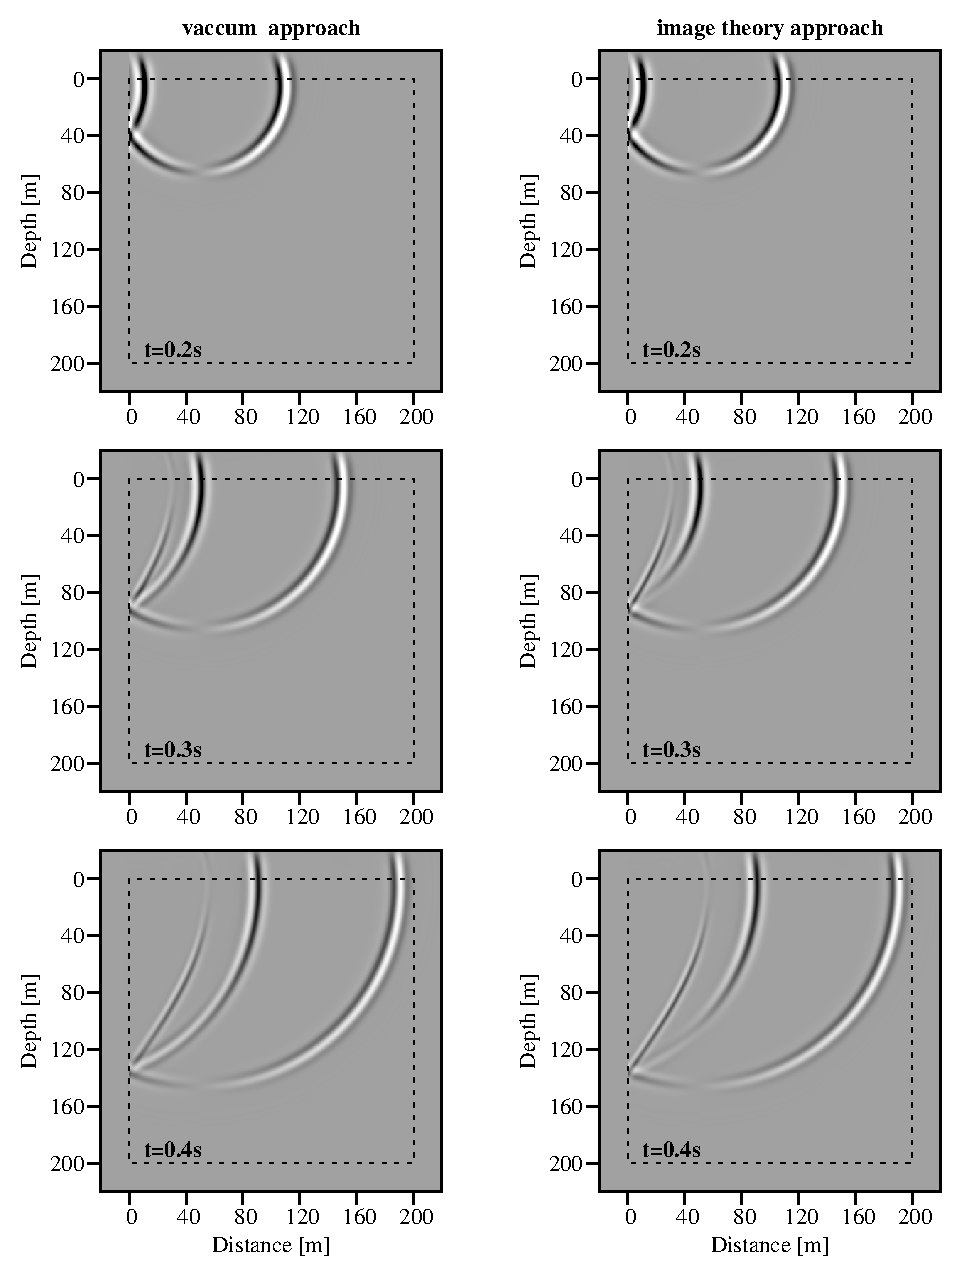
\includegraphics[scale=1.0]{fig/validation_fsurf.eps}
  \caption{Two possible approach to implement free surface: (left) the vacuum approach and (right) the image theory approach.}
\end{figure}

\section{Sources}
\index{sources}

\subsection{Explosive source}
\index{explosive source}

\noindent Explosive source is added to normal stress $\sigma_{xx}$ and $\sigma{zz}$.

\subsection{Body force source}
\index{force source}



% ----------------------------------------------------------------------
% GETTING STARTED
% ----------------------------------------------------------------------
\chapter{Getting started}

\section{Requirements}

\noindent For FDPSV program:
\begin{itemize}
	\item GNU make $>=$ 4.1
	\item GNU gfortran $>=$ 4.7
\end{itemize}

\noindent Optional for examples:
\begin{itemize}
	\item python $>=$ 2.7
	\item python-numpy $>=$ 1.8.2
\end{itemize}

\noindent Optional:
\begin{itemize}
	\item Seismic Un*x $>=$ 43R1
\end{itemize}

\subsection{Compilation}
\addbash{make}

% ----------------------------------------------------------------------
% INPUT PARAMETERS AND FILES
% ----------------------------------------------------------------------
\section{Input parameters and files}
\index{input parameters}
\index{input files}

% ----------------------------------------------------------------------
% NUMERICAL EXAMPLES
% ----------------------------------------------------------------------
\chapter{Numerical examples}

\section{Weathered model}

\section{Corner-edge model}

\section{Advanced model}


% ----------------------------------------------------------------------
% APPENDICES
% ----------------------------------------------------------------------
\begin{appendices}
%\chapter{Finite-difference equations}
\index{finite-difference equations}
\chapter{Finite-difference equations}

\begin{equation}
  E(i,j)=\lambda(i,j)+2\mu (i,j)
\end{equation}

\begin{eqnarray}
  D_{t}^{+}v_{x}^{t}({\scriptstyle i,j+1/2,l-1/2}) = \rho_{x}^{-1}({\scriptstyle i,j}) [D_{x}^{+}\tau_{xx}({\scriptstyle i,j,l})+D_{z}^{-}\tau_{xz}({\scriptstyle i+1/2,j,l})] \\
  D_{t}^{+}v_{z}^{t}({\scriptstyle i+1/2,j,l-1/2}) = \rho_{z}^{-1}({\scriptstyle i,j}) [D_{x}^{-}\tau_{xz}({\scriptstyle i+1/2,j+1/2,l})+D_{z}^{+}\tau_{zz}({\scriptstyle i,j,l})] \\
  D_{t}^{+}\tau_{xx}({\scriptstyle i,j,l}) = E({\scriptstyle i,j}) D_{x}^{-}v_{x}({\scriptstyle i,j+1/2,l+1/2})+\mu({\scriptstyle i,j}) D_{z}^{-}v_{z}({\scriptstyle i+1/2,j,l+1/2}) \\
  D_{t}^{+}\tau_{zz}({\scriptstyle i,j,l}) = \mu({\scriptstyle i,j}) D_{x}^{-}v_{x}({\scriptstyle i,j+1/2,l+1/2})+ E({\scriptstyle i,j}) D_{z}^{-}v_{z}({\scriptstyle i+1/2,j,l+1/2})\\
  D_{t}^{+}\tau_{xz}({\scriptstyle i+1/2,j+1/2,l}) = \bar{\mu}({\scriptstyle i+1/2,j+1/2})[D_{z}^{+}v_{x}({\scriptstyle i,j+1/2,l+1/2}) +D_{x}^{+}v_{z}({\scriptstyle i+1/2,j,l+1/2})]  
\end{eqnarray}


%\chapter{GNU Free Documentation License}
\index{GNU FDL}  
\input{fdl-1.3}

\end{appendices}
  
% ----------------------------------------------------------------------
% References
% ----------------------------------------------------------------------

\bibliography{references,bibmanual}

\clearpage
\newpage
\thispagestyle{empty}
\printindex

\end{document}
